\documentclass{article}

\usepackage{float}
% \usepackage{floatrow}
\usepackage[T1, T2A]{fontenc}
\usepackage[english, serbian c]{babel}
\usepackage[utf8]{inputenc}
\usepackage{xcolor}

\usepackage[a4paper, total={6in, 8in}]{geometry}

\usepackage{amsmath}
\usepackage{graphicx}
\usepackage[colorlinks=true, allcolors=blue]{hyperref}

\usepackage{hyperref}
\hypersetup{colorlinks,linkcolor={black},citecolor={blue},urlcolor={blue}}  

\title{\textbf{ИНФОРМАЦИОНИ СИСТЕМИ} \\
\vspace{10}
\Large{\textbf{АЕРОДРОМ}}}
\author{Тамара Томић, 1046/2023 \\ \textit{mi231045@alas.matf.bg.ac.rs} \\\\
        Тамара Ђукић, 1051/2023 \\ \textit{mi231051@alas.matf.bg.ac.rs} \\\\
        Тамара Јевтимијевић, 1045/2023 \\ \textit{mi231045@alas.matf.bg.ac.rs} \\\\
        Милош Милаковић, 1052/2021 \\ \textit{mi211052@alas.matf.bg.ac.rs}}
\date{Новембар 2023.}
\begin{document}

\maketitle

\vspace{17}
\begin{figure}[h!]
    \centering
    \includegraphics[width=4cm, height=4cm]{grb.png}
\end{figure} 

\newpage
\tableofcontents

\newpage

\section{Увод}

\section{Анализа система}

\section{Процеси и случајеви употребе}

\subsection{Административни случајеви употребе}

\subsubsection{Уношење авиона у систем}

\subsubsection{Брисање авиона ис система}

\subsection{Резервација аеродрома (писте):}
\begin{itemize}
\item \textbf{Кратак опис:} Авио компанија контактира са администратором аеродрома задуженим за резервације писте у циљу резервисања писте за полетање или слетање својих авиона. Са администратором може да се договара око датума, времена као и цене резервисања писте.
\item \textbf{Учесници:}
\begin{itemize}
    \item Авио компанија;
    \item Администратор који је задужен за резервације писте.
\end{itemize}
 \item \textbf{Предуслови:} Авио компанија поседује барем један авион и да је регистрована тј. да има уговор о пословању са аеродромом.
 \item \textbf{Постуслови:} Авио компанија или јесте или није резервисала писту.
 \item \textbf{Основни ток:}
 \begin{enumerate}
    \item Авио компанија пише захтев за резервацију аеродрома у ком наводи тачно време и тачну адресу кад жели да резервише писту.
    \item Када је написала захтев, шаље га администратору аеродрома, који је задужен за резервације писте.
    \item Администратор проверава доступност писте и шаље одговор авио компанији.
    \begin{enumerate}
        \item Ако је одговор негативан
        \begin{itemize}
            \item Авио компанија отказује резервацију.
            \item Авио компанија мења датум и време и то шаље администратору.
        \end{itemize}
        \item Ако је одговор позитиван, администратор шаље авио компанији цену резервације писте за тај термин.
    \end{enumerate}
    \item Авио компанија разматра цену и обавештава администратора да ли цена одговара или не.
     \begin{enumerate}
        \item Ако цена не одговара 
        \begin{itemize}
            \item Авио компанија отказује резервацију.
            \item Авио компанија мења датум и време и то шаље администратору.
        \end{itemize}
        \item Ако цена одговара, администратор врши резервацију писте.
    \end{enumerate}
    \item Комуникације између администратора и авио компаније је завршена.
\end{itemize}
 
\begin{figure}[H]
    \centering
    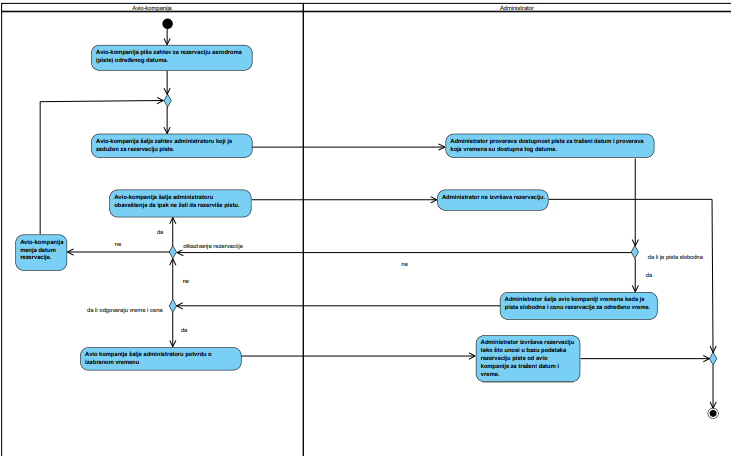
\includegraphics[width=16cm, height=17cm]{Dijagrami_slike/rezervacija_aerodroma.png}
    \caption{Дијаграм активности - Резервација аеродрома (писте)}
\end{figure}

\subsection{Праћење летова}

\subsection{Обрада захтева}

\subsubsection{Чекирање путника}

\subsubsection{Чекирање запослених}

\subsection{Одржавање авиона}

\subsubsection{Пријава квара}

\subsubsection{Поправка квара}

\subsubsection{Уношење потребних делова у систем}

\section{База података}

\section{Софтверска архитектура}

\section{Кориснички интерфејс}


\end{document}